% Standalone XeLaTeX. Original: 2014ap_exam.pdf, PDF pp.14--15.
\documentclass[11pt,a4paper]{article}
\usepackage[margin=23mm]{geometry}
\usepackage{fontspec}
\usepackage{xeCJK}
\setCJKmainfont{HaranoAjiMincho-Regular.otf}
\setCJKsansfont{HaranoAjiGothic-Medium.otf}
\usepackage{amsmath,amssymb}
\usepackage{tikz}
\usetikzlibrary{arrows.meta}
\renewcommand{\figurename}{図}
\setlength{\parindent}{1em}
\setlength{\parskip}{0.35em}
\title{物理工学専攻 院試解答集 ver2\\2014年 物理学II 第4問}
\author{政岡凜太郎}
\date{}
\begin{document}
\maketitle

\section*{[1] 逆格子と第一ブリュアン域}
逆格子の定義は $\boldsymbol a_i\cdot\boldsymbol b_j=2\pi\delta_{ij}$ である。$\boldsymbol b_1=(u,v)$ とすると
\[
 \frac{\sqrt3a}{2}u+\frac a2v=2\pi,
 \qquad -\frac{\sqrt3a}{2}u+\frac a2v=0.
\]
和と差から $v=2\pi/a$, $u=2\pi/(\sqrt3a)$ を得る。同様に
\begin{equation}
 \boxed{\boldsymbol b_1=2\pi\left(\frac{1}{\sqrt3a},\frac1a\right),\qquad
 \boldsymbol b_2=2\pi\left(-\frac{1}{\sqrt3a},\frac1a\right).}
\end{equation}
第一ブリュアン域は、原点と最短の逆格子点との垂直二等分線に囲まれた領域である。最短の6点は
$\pm\boldsymbol b_1,\pm\boldsymbol b_2,\pm(\boldsymbol b_1-\boldsymbol b_2)$。
各境界は $\boldsymbol k\cdot\boldsymbol G=|\boldsymbol G|^2/2$ を満たす。
$\boldsymbol G=\boldsymbol b_1-\boldsymbol b_2$ の境界は $k_x=2\pi/(\sqrt3a)$。
$\boldsymbol b_1,\boldsymbol b_2$ の境界の交点は $k_x=0$, $k_y=4\pi/(3a)$ なので
\begin{equation}
 \boxed{P=\left(\frac{2\pi}{\sqrt3a},0\right),\qquad
 Q=\left(0,\frac{4\pi}{3a}\right).}
\end{equation}
得られる領域は図の正六角形である。図中のOは波数原点を表す。

\section*{[2] スピンを含めた自由電子の状態数}
単位胞の面積を $s$、系全体の面積を $S$ とすると
\[
 s=|\boldsymbol a_1\times\boldsymbol a_2|=\frac{\sqrt3}{2}a^2,
 \qquad \text{電子数}=\frac{2S}{s}.
\]
波数空間で単位面積あたりの状態数は $S/(2\pi)^2$。スピン2重を含めて円内の状態を数えると
\begin{equation}
 2\frac{S}{(2\pi)^2}\pi k_F^2=\frac{2S}{s},
 \qquad \boxed{k_F=\frac1a\sqrt{\frac{8\pi}{\sqrt3}}.}
\end{equation}

\section*{[3] フェルミ面と第一域の関係}
円の面積は $\pi k_F^2=(2\pi)^2/s$ で、第一ブリュアン域の面積に等しい。
ただし形は円と六角形で異なる。六角形の内接半径 $r_{\rm in}$ と外接半径 $r_{\rm out}$ は
\[
 r_{\rm in}=\frac{2\pi}{\sqrt3a},\qquad
 r_{\rm out}=\frac{4\pi}{3a},\qquad r_{\rm in}<k_F<r_{\rm out}.
\]
したがってフェルミ面は各辺を横切るが、六角形の頂点には届かない。自由電子の仮定ではこの円を切り詰めずに描く。
\begin{figure}[htbp]
\centering
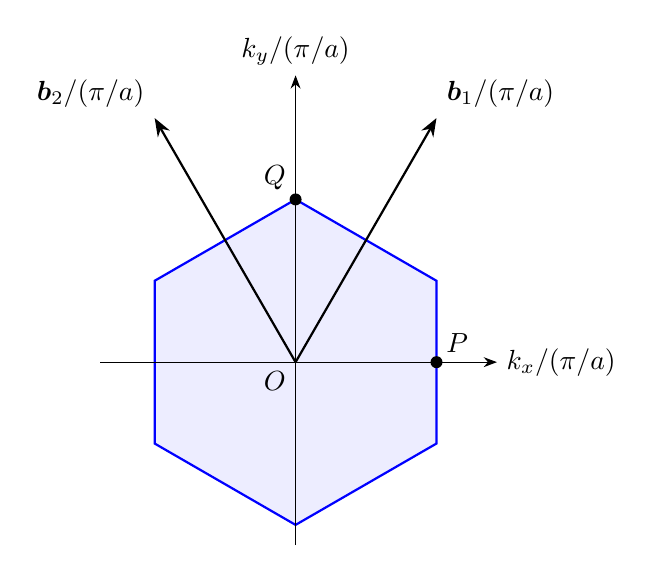
\begin{tikzpicture}[>=Stealth,scale=1.55]
 \pgfmathsetmacro{\px}{2/sqrt(3)}
 \pgfmathsetmacro{\qy}{4/3}
 \pgfmathsetmacro{\sy}{\qy/2}
 \fill[blue!7] (0,\qy)--(\px,\sy)--(\px,-\sy)--(0,-\qy)--(-\px,-\sy)--(-\px,\sy)--cycle;
 \draw[thick,blue] (0,\qy)--(\px,\sy)--(\px,-\sy)--(0,-\qy)--(-\px,-\sy)--(-\px,\sy)--cycle;
 \draw[->] (-1.6,0)--(1.65,0) node[right] {$k_x/(\pi/a)$};
 \draw[->] (0,-1.5)--(0,2.35) node[above] {$k_y/(\pi/a)$};
 \draw[->,thick] (0,0)--(\px,2) node[above right] {$\boldsymbol b_1/(\pi/a)$};
 \draw[->,thick] (0,0)--(-\px,2) node[above left] {$\boldsymbol b_2/(\pi/a)$};
 \fill (\px,0) circle(1.4pt) node[above right] {$P$};
 \fill (0,\qy) circle(1.4pt) node[above left] {$Q$};
 \node[below left] at (0,0) {$O$};
\end{tikzpicture}
\hspace{5mm}
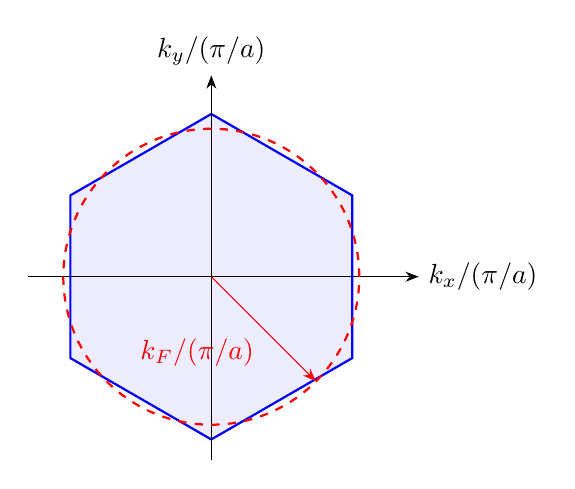
\begin{tikzpicture}[>=Stealth,scale=1.55]
 \pgfmathsetmacro{\px}{2/sqrt(3)}
 \pgfmathsetmacro{\qy}{4/3}
 \pgfmathsetmacro{\sy}{\qy/2}
 \pgfmathsetmacro{\kf}{sqrt(8/(pi*sqrt(3)))}
 \fill[blue!7] (0,\qy)--(\px,\sy)--(\px,-\sy)--(0,-\qy)--(-\px,-\sy)--(-\px,\sy)--cycle;
 \draw[thick,blue] (0,\qy)--(\px,\sy)--(\px,-\sy)--(0,-\qy)--(-\px,-\sy)--(-\px,\sy)--cycle;
 \draw[->] (-1.5,0)--(1.7,0) node[right] {$k_x/(\pi/a)$};
 \draw[->] (0,-1.5)--(0,1.65) node[above] {$k_y/(\pi/a)$};
 \draw[red,thick,dashed] (0,0) circle(\kf);
 \draw[->,red] (0,0)--({\kf/sqrt(2)},{-\kf/sqrt(2)}) node[midway,below left] {$k_F/(\pi/a)$};
\end{tikzpicture}
\caption{左: 逆格子と第一域。座標の単位は $\pi/a$。右: 同じ縮尺の第一域（青線）と自由電子のフェルミ面（赤破線）。}
\end{figure}

\section*{[4] 原子軌道への射影}
原問の図2の配置に従って、Aから最近接Bへの変位を
\begin{equation}
 \boldsymbol\delta_1=\frac{\boldsymbol a_1+2\boldsymbol a_2}{3},\quad
 \boldsymbol\delta_2=\frac{\boldsymbol a_1-\boldsymbol a_2}{3},\quad
 \boldsymbol\delta_3=\frac{-2\boldsymbol a_1-\boldsymbol a_2}{3}
\end{equation}
と選ぶ。どれも長さ $a/\sqrt3$ である。最近接位相の和を
\[
 f(\boldsymbol k)=\sum_{j=1}^3 e^{i\boldsymbol k\cdot\boldsymbol\delta_j}
\]
と定義する。以下 $\lambda^A=\lambda^A_{\boldsymbol k}$, $\lambda^B=\lambda^B_{\boldsymbol k}$ と略記する。
A軌道への固有方程式の射影は、規格化積分と最近接行列要素だけを残して
\begin{align}
 \int\phi_A(\boldsymbol r-\boldsymbol r_i^A)\mathcal H\psi_{\boldsymbol k}(\boldsymbol r)\,\mathrm d\boldsymbol r
 &=e^{i\boldsymbol k\cdot\boldsymbol r_i^A}
   [\epsilon_A\lambda^A+\tau f(\boldsymbol k)\lambda^B],\\
 E(\boldsymbol k)\int\phi_A(\boldsymbol r-\boldsymbol r_i^A)\psi_{\boldsymbol k}(\boldsymbol r)\,\mathrm d\boldsymbol r
 &=e^{i\boldsymbol k\cdot\boldsymbol r_i^A}E(\boldsymbol k)\lambda^A.
\end{align}
BからAへの最近接変位は $-\boldsymbol\delta_j$ なので、Bへの射影には $f^*$ が現れる。
共通の位相を除くと
\begin{equation}
 \boxed{\begin{pmatrix}\epsilon_A&\tau f(\boldsymbol k)\\\tau f(\boldsymbol k)^*&\epsilon_B\end{pmatrix}
 \begin{pmatrix}\lambda^A\\\lambda^B\end{pmatrix}
 =E(\boldsymbol k)\begin{pmatrix}\lambda^A\\\lambda^B\end{pmatrix}.}
\end{equation}
これは係数に対する方程式であり、原本のBloch和全体の規格化を仮定する必要はない。

\section*{[5] 二本のエネルギー帯}
行列式がゼロになる条件は
\[
 (E-\epsilon_A)(E-\epsilon_B)-\tau^2|f(\boldsymbol k)|^2=0.
\]
したがって上帯を $E_+$、下帯を $E_-$ とすると
\begin{equation}
 \boxed{E_\pm(\boldsymbol k)=\frac{\epsilon_A+\epsilon_B}{2}
 \pm\sqrt{\frac{(\epsilon_A-\epsilon_B)^2}{4}+\tau^2|f(\boldsymbol k)|^2}.}
\end{equation}
位相の和の絶対値の二乗は
\begin{align}
 |f|^2&=3+2\sum_{i<j}\cos[\boldsymbol k\cdot(\boldsymbol\delta_i-\boldsymbol\delta_j)]\\
 &=3+4\cos\left(\frac{\sqrt3a k_x}{2}\right)\cos\left(\frac{a k_y}{2}\right)
       +2\cos(a k_y).
\end{align}
よってこの最後の式を代入すれば $k_x,k_y$ の明示的な関数になる。

\section*{[6] 占有状態と最小ギャップ}
各エネルギー帯は単位胞あたりスピン込みで2個の電子を収容する。
電子が単位胞あたり2個なら下帯は満たされ、上帯は空である。
$f=0$ で下帯が最大、上帯が最小となる。
$k_x=0$ では
\[
 |f|^2=1+4\cos\left(\frac{ak_y}{2}\right)+4\cos^2\left(\frac{ak_y}{2}\right)
       =\left[1+2\cos\left(\frac{ak_y}{2}\right)\right]^2.
\]
ゼロになるのは $\cos(ak_y/2)=-1/2$。第一域にある点は
\begin{equation}
 \boxed{X=\left(0,\pm\frac{4\pi}{3a}\right),\qquad
 E_1=\epsilon_B,\quad E_2=\epsilon_A,\quad E_g=\epsilon_A-\epsilon_B.}
\end{equation}
これらは図の上・下の頂点に当たる。以下では $X=(0,4\pi/(3a))$ を選ぶ。

\section*{[7] X近傍の曲率と有効質量}
$k_y=4\pi/(3a)+q$ とおき、$|aq|\ll1$ で展開すると
\[
 1+2\cos\left(\frac{2\pi}{3}+\frac{aq}{2}\right)
 =-\frac{\sqrt3a}{2}q+O(q^2).
\]
$E_g>0$ なので平方根を展開できる。原問の $E_g\gg|\tau|$ の範囲では
\begin{align}
 E_+(q)&=\epsilon_A+\frac{3a^2\tau^2}{4E_g}q^2+O(q^3),\\
 E_-(q)&=\epsilon_B-\frac{3a^2\tau^2}{4E_g}q^2+O(q^3).
\end{align}
電子の有効質量を $1/m^*=(1/\hbar^2)\,\partial^2 E/\partial k_y^2$ で定義すると
\begin{equation}
 \boxed{m^*_+=\frac{2\hbar^2 E_g}{3a^2\tau^2},\qquad
 m^*_-=-\frac{2\hbar^2 E_g}{3a^2\tau^2}.}
\end{equation}
上帯は極小なので正、下帯は極大なので負である。下帯のホールを用いる場合は、電子の符号付き曲率質量とは別に $m^*_{\rm hole}=|m^*_-|$ となる。

\clearpage
\section*{[8] すべて同じ原子にした場合}
$\epsilon_B=\epsilon_A$ とするとギャップは消え、$k_x=0$ で
\[
 E_\pm(k_y)=\epsilon_A\pm|\tau|\left|1+2\cos\left(\frac{ak_y}{2}\right)\right|.
\]
よってX近傍では
\begin{equation}
 \boxed{E_\pm(q)=\epsilon_A\pm\frac{\sqrt3a|\tau|}{2}|q|+O(q^2),\qquad E_g=0.}
\end{equation}
上下のエネルギーを大小で並べると $|q|$ を含む直線的な交差になる。
[7]の放物的な有効質量の式を、ギャップが消える場合にそのまま用いることはできない。
\end{document}
